\section{Introduction}
Dans un monde où l'informatique et la virtualisation des environnements de
travail est omniprésente, la visualisation des données est devenu un enjeux
primordiale pour des domaines aussi variés que la médecine, l'architecture,
l'industrie du jeux vidéo ou encore les interfaces utilisateur.

\paragraph{\eng{Rasterisation}}
Encore aujourd'hui, la méthode privilégiée de visualisation des environnements
3D est la \eng{rasterisation}. Cette technique consiste à modéliser
l'\tsl{univers}\footnote{Au sens mathématique, \ie tout ce qui est contenu
dans un système en troi dimensions.} par un ensemble de triangles. Ces
triangles sont transformé (\ie translatés, mis à l'échelle, \etc) puis projeté
dans un monde plan : Notre écran. La \fref{rasterisationPipeline} représente
grossièrement le cheminement des données jusqu'à l'image finale.

\begin{figure}[H]
\begin{center}
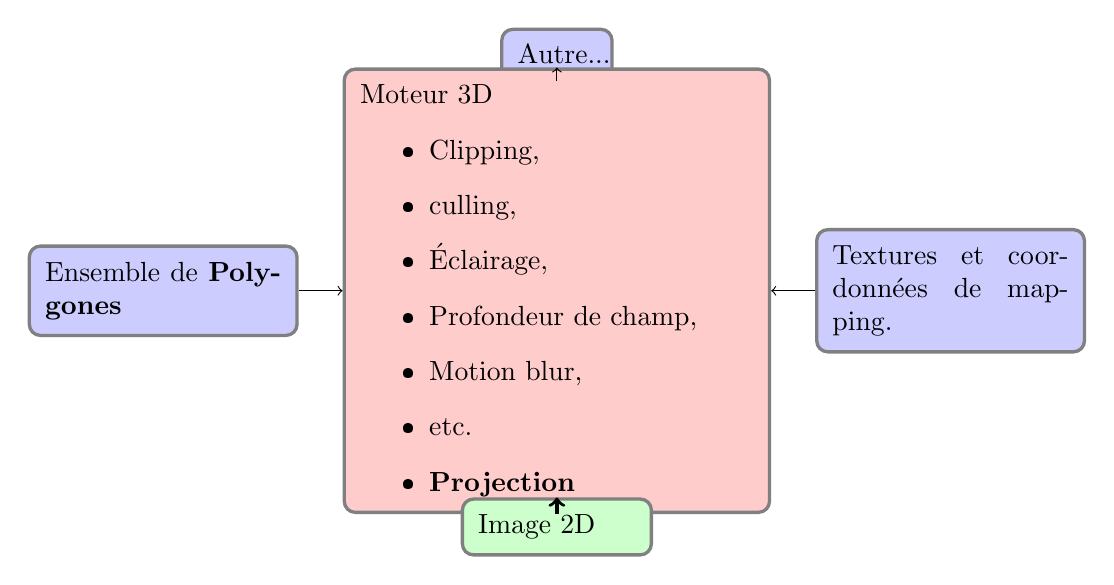
\begin{tikzpicture}
  [entree/.style={
    draw=black!50,
    fill=blue!20,
    rectangle,
    rounded corners,
    inner sep=.2cm,
    very thick}, systeme/.style={
    draw=black!50,
    fill=red!20,
    rectangle,
    rounded corners,
    inner sep=.2cm,
    very thick}, sortie/.style={
    draw=black!50,
    fill=green!20,
    rectangle,
    rounded corners,
    inner sep=.2cm,
    very thick}]

  \node [entree] at (-5,0) (polygone) {
  \begin{minipage}{3cm}
    Ensemble de \textbf{Polygones}
  \end{minipage}
  };

  \node [entree] at (5,0) (textures) {
  \begin{minipage}{3cm}
    Textures et coordonnées de mapping.
  \end{minipage}
  };

  \node [entree] at (0,3) (other) {
  \begin{minipage}{1cm}
    Autre...
  \end{minipage}
  };

  \node [systeme] (engine) {
  \begin{minipage}{5cm}
    Moteur 3D 
    \begin{itemize}
      \item Clipping,
      \item culling,
      \item Éclairage,
      \item Profondeur de champ,
      \item Motion blur,
      \item etc.
      \item \textbf{Projection}
    \end{itemize}
  \end{minipage}
  };

  \node [sortie] at (0,-3) (image) {
  \begin{minipage}{2cm}
    Image 2D
  \end{minipage}
  };

  \draw [->] (polygone) -- (engine);
  \draw [->] (textures) -- (engine);
  \draw [->] (other) -- (engine);
  \draw [very thick, ->] (engine) -- (image);
\end{tikzpicture}
\caption{Représentation grossière du pipeline de rendu via la
rasterisation\label{rasterisationPipeline}}
\end{center}

\end{figure}


L'avantage de cette technique vient du fait que les calculs sont très
aisément parallélisables. Nous assistons d'ailleurs à un développement de
technologie dans ce sens : Les \gls{GPU} sont devenu de vraies collections de
processeurs.

\newpar Mais cette technique n'offre pas que des avantages. En effet, la
compleification des scènes en 3D et surtout la demande du publique pour des
rendu encore plus réaliste pousse dans ses retranchement le matériel et les
logiciels de visualisation 3D. Mais depuis quelques plus de 30 ans
\cite{Whitted1980}, chercheurs et ingénieurs développent une technique de
rendu simple mais très puissante : Le \raytracing !

\subsection{Le \raytracing ?}
Le \raytracing est une technique de rendu qui, à la manière des réseau de
neurones, tente de s'approcher au plus des phénomènes physique pour obtenir
un rendu photoréaliste. 

\newpar À défaut de décrire le \tsl{pipeline} complet d'un ray tracer (ce
n'est pas l'objectif du rapport), il m'a tout de même semblé important
d'écrire une brève introduction sur ce qui pourrait bien être la principale
méthode de rendu dans un futur proche.

\paragraph{Le modèle de propagation de la lumière}
L'œil humain perçoit les objets grâce à la lumière qu'ils réfléchissent. Nous
pourrions donc imaginer calculer l'ensemble des interactions lumineuse d'un
scène en partant de toutes les sources de lumière. Un tel modèle supposerai
cependant une puissance de calcul infinie et pour que les calculs restent
raisonnable, les simplifications suivantes ont dû être faite :
\begin{itemize}
  \item La lumière se propage en ligne droite : Nous abandonnons donc le
    modèle ondulatoire de la lumière pour nous restreindre à l'optique
    géométrique.
  \item La lumière que nous recevons est la même que si la source était notre
    œil : En effet, plutôt que de lancer la majorité des rayons dans le vide
    (\ie des rayons qui ne parviendraient pas jusqu'à notre œil), il est plus
    judicieux de lancer les rayons depuis la caméra jusqu'à notre scène.
  \item Le nombre de rebond que fait la lumière est fini : En optique
    géométrie, il n'y a pas de perte d'énergie et considérer tous les rebonds
    mènerai à des récursions infinies.
\end{itemize}

\paragraph{L'algorithme simplifié}
Cette courte introduction nous amène à l'algorithme de rendu suivant :
\begin{algorithm}[H]
\caption{getPixel}
\begin{algorithmic}
\REQUIRE X, l'abscisse du point dont on veux la couleur.
\REQUIRE Y, l'ordonnée du point dont on veux la couleur.
\REQUIRE L, le niveau de récursion, \ie le nombre de fois que le rayon a été
réfléchi ou réfracté.
\ENSURE La couleur du pixel demandé.

\STATE FinalColor $\leftarrow$ BLACK
\IF {L $\gt$ MAX\_RECURSION\_LEVEL}
  \RETURN FinalColor
\ENDIF
\STATE
\STATE Ray $\leftarrow$ Camera.getRay (X, Y)
\STATE Record $\leftarrow$ getClosestHit ( Ray )
\STATE
\IF {Hit}
 \IF{La surface est réfléchissante}
    \STATE Lancer le rayon réfléchi.
 \ENDIF

 \IF{La surface est transparente}
    \STATE Lancer le rayon transmis.
 \ENDIF
 \STATE
 \STATE FinalColor $\leftarrow$ Couleur ambiente + 
  Contribution Lumineuse * (Couleur de l'objet + Couleur du rayon transmis +
  Couleur du rayon réfléchi)
\ENDIF
\STATE
\RETURN FinalColor
\end{algorithmic}
\end{algorithm}


\todo{Intégrer l'image}

Il est impressionnant de constater la simplicité d'un algorithme pourtant si
puissant. En quelques lignes, nous venons de décrire la propagation de la
lumière aux travers d'objets transparents et/ou réfléchissant !

Nous verrons cependant que, pour rester ouvert à l'extension et garder un
couplage faible, une architecture solide est nécessaire.

\chapter{Objectifs}
Les objectifs du projet sont nombreux, aussi bien sur le plan de
l'architecture logiciel, que de la gestion de projet, de la rédaction ou
encore du développement.

\paragraph{Architecture logiciel -} Un des principaux buts du projet (si ce
n'est le but principal du projet) est de créer un programme ouvert à
l'extension et pouvant servir de base à la création d'un \eng{raytracer}\ plus
évolué, plus rapide, ou plus facile à utiliser.

L'architecture du programme est défini à la section \ref{sec:architecture}.

\paragraph{Portabilité -} Afin d'être le plus portable possible, j'ai décidé
d'utiliser un ensemble d'outils standards et libres :
\begin{itemize}
  \item \tsl{Le langage C++ :}\ \eng{Open-Spec}\ et compilable sur presque
    toutes les plateformes.
  \item \tsl{Les autotools}\footnote{\url{http://sources.redhat.com/autobook/}
    :}\ Système de build standard et ne nécessitant aucun autre programme que
    make et bash. De plus, il assure une portabilité maximale en vérifiant la
    présence de toutes les bibliothèques nécessaire à la compilation et au bon
    fonctionnement du programme.
  \item \tsl{Boost :}\ La bibliothèque C++ de référence.
  \item \tsl{libpng/libjpg :}\ Pour l'import texture et l'export des résultats.
  \item \tsl{lib3ds :}\ Pour l'importation des modèles 3D.
  \item \tsl{\LaTeX{} :}\ Pour la rédaction du rapport.\\

  \item \tsl{Tim Horton :}\ Pour le café et les beignets.
\end{itemize}

\paragraph{Gestion de projet -} J'ai réalisé ce projet seul du 24 Septembre au
1 Décembre en utilisant un style de développement
\gls{XP}\footnote{\url{http://www.extremeprogramming.org/}}.  Le gestionnaire
de version utilisé est \tsl{git}\ et le projet ainsi que son
\href{http://digitalguru.github.com/LyonRayTracer}{site web} sont hébergés sur
\href{http://github.com}{GitHub}.

\remark{Parce que la charge de travail aurait été trop grande, j'ai décidé de
ne pas rédiger les documents de références du type \tsl{Dossier
d'initialiation}, \tsl{Dossier de jalonnage}, \tsl{Planning prévisionnel},
\etc J'ai cependant pris soin de rédiger une documentation exhaustive de
chacune des classes du projet.}
\vspace*{1em}

\paragraph{Implémentation -} Il était pour moi primordial de respecter tout au
long de ce projet des \eng{guidelines}\ afin d'assurer une cohérence de tout
le code (plusieurs milliers de lignes tout de même). J'ai pour cela suivit
principalement le guide de style définit par Herb \tsc{Sutter} dans
\cite{Sutter05}. Je me suis aussi inspiré de \cite{Meyers94}.\\

Enfin, la documentation fait aussi partie intégrante du processus de
développement et la génération de celle-ci fait partie du \eng{pipeline} de
compilation.

\paragraph{Fonctionnalité du ray tracer -} Reprenons les objectifs fixés dans
le sujet :
\begin{enumerate}
  \item \tickmark{} Un moteur de \raytracing\ ``classique''.
  \item \tickmark{} La gestion de primitives (sphères, plan, boite,
    triangles).
  \item \tickmark{} La gestion de plusieurs types de caméras : Orthographique,
    perspective, \etc
  \item \tickmark{} La gestion de plusieurs types de lumières : Point, plane,
    directionnelle, \etc
  \item \tickmark{} La gestion d'au moins un format de représentation
    polygonale.
  \item \tickmark{} La mise en place des structures accélératrices.
  \item \tackmark{} La gestion du \eng{photon mapping} : Comme je l'avais
    pressentie dans mon sujet, le temps alloué au projet était insuffisant
    pour l'implémentation d'une telle fonctionnalité.\\
\end{enumerate}

J'ai cependant pris le temps d'implémenter en plus :
\begin{enumerate}
  \item Un chargeur de scènes XML.
  \item La lecture et l'écriture d'images au format PNG ou JPG (avec la
    possibilité d'ajouter d'autre formats).
  \item La gestion des textures.
  \item Le \gls{supersampling}.
  \item La gestion des ombres douces.
  \item La gestion de la profondeur de champ.
\end{enumerate}

\subsection{Non-objectifs}
Comme dans tout projet, celui-ci possède des non-objectifs, \ie des objectifs
que j'ai volontairement choisi de ne pas atteindre, ou en tout cas de ne pas
viser.\\

D'abord, concernant la vitesse d'exécution. Les \eng{raytracers} commerciaux
sont de réelles prouesses d'ingénierie et d'optimisation et j'ai considéré que
l'optimisation de mon programme sortait du contexte d'un projet personnel.\\

Il ne s'agissait pas non plus d'en faire un produit fini mais plutôt un
\tsl{proof of concept}. Il reste donc de nombreuses améliorations tant au
niveaux des fonctionnalités existantes qu'au niveau de celles à ajouter.
 % CHECKED

\subsection{Non-objectifs}
Comme dans tout projet, celui-ci possède des non-objectifs, \ie des objectifs
que j'ai volontairement choisi de ne pas atteindre, ou en tout cas de ne pas
viser.\\

D'abord, concernant la vitesse d'exécution. Les \eng{raytracers} commerciaux
sont de réelles prouesses d'ingénierie et d'optimisation et j'ai considéré que
l'optimisation de mon programme sortait du contexte d'un projet personnel.\\

Il ne s'agissait pas non plus d'en faire un produit fini mais plutôt un
\tsl{proof of concept}. Il reste donc de nombreuses améliorations tant au
niveaux des fonctionnalités existantes qu'au niveau de celles à ajouter.

